\documentclass[conference]{IEEEtran}

% *** PDF, URL AND HYPERLINK PACKAGES ***
%
%\usepackage{url}
% url.sty was written by Donald Arseneau. It provides better support for
% handling and breaking URLs. url.sty is already installed on most LaTeX
% systems. The latest version and documentation can be obtained at:
% http://www.ctan.org/pkg/url
% Basically, \url{my_url_here}.

% for figures
\usepackage{graphicx}


\begin{document}
%
% paper title
% Titles are generally capitalized except for words such as a, an, and, as,
% at, but, by, for, in, nor, of, on, or, the, to and up, which are usually
% not capitalized unless they are the first or last word of the title.
% Linebreaks \\ can be used within to get better formatting as desired.
% Do not put math or special symbols in the title.
\title{Magic Mirror Web Interface\\ Using the Raspberry PI}

% author names and affiliations
% use a multiple column layout for up to three different
% affiliations
\author{\IEEEauthorblockN{Michael Meding}
\IEEEauthorblockA{University of Massachusetts Lowell\\Computer Science\\
Lowell, Massachusetts 01852\\
Email: mike@mikemeding.com}
\and
\IEEEauthorblockN{Peter Welby}
\IEEEauthorblockA{University of Massachusetts Lowell\\Computer Science\\
Lowell, Massachusetts 01852\\
Email: pwelby@cs.uml.edu}
\and
\IEEEauthorblockN{Harun Guna}
\IEEEauthorblockA{University of Massachusetts Lowell\\Computer Science\\
Lowell, Massachusetts 01852\\
Email: harung1993@gmail.com}
}



% make the title area
\maketitle

% As a general rule, do not put math, special symbols or citations
% in the abstract
\begin{abstract}
This semesters IoT project was building a “Magic Mirror”. 
A Magic Mirror is a piece of 1 way glass with a computer monitor behind it to display a set of dynamic information such as the news, weather, or personal calendar events in the presence of person in front of it.
\end{abstract}


\section{Introduction}
%A brief introduction to the background, motivation of the work, challenges of performing the work, contributions of the work and the structure of the rest of the paper. Novelty of the work should be emphasized in the section of introduction.
A Magic Mirror is a Raspberry Pi powered computer display that sits behind a sheet of one way mirror glass as shown in Figure \ref{fig:mirror}.
The Mirror is designed to detect the presence of person and activate the display when a person is detected.
Displayed on the screen are various dynamic items which the user may find helpful when looking in the mirror such as the current weather and time.
\begin{figure}[!ht]
  \centering
  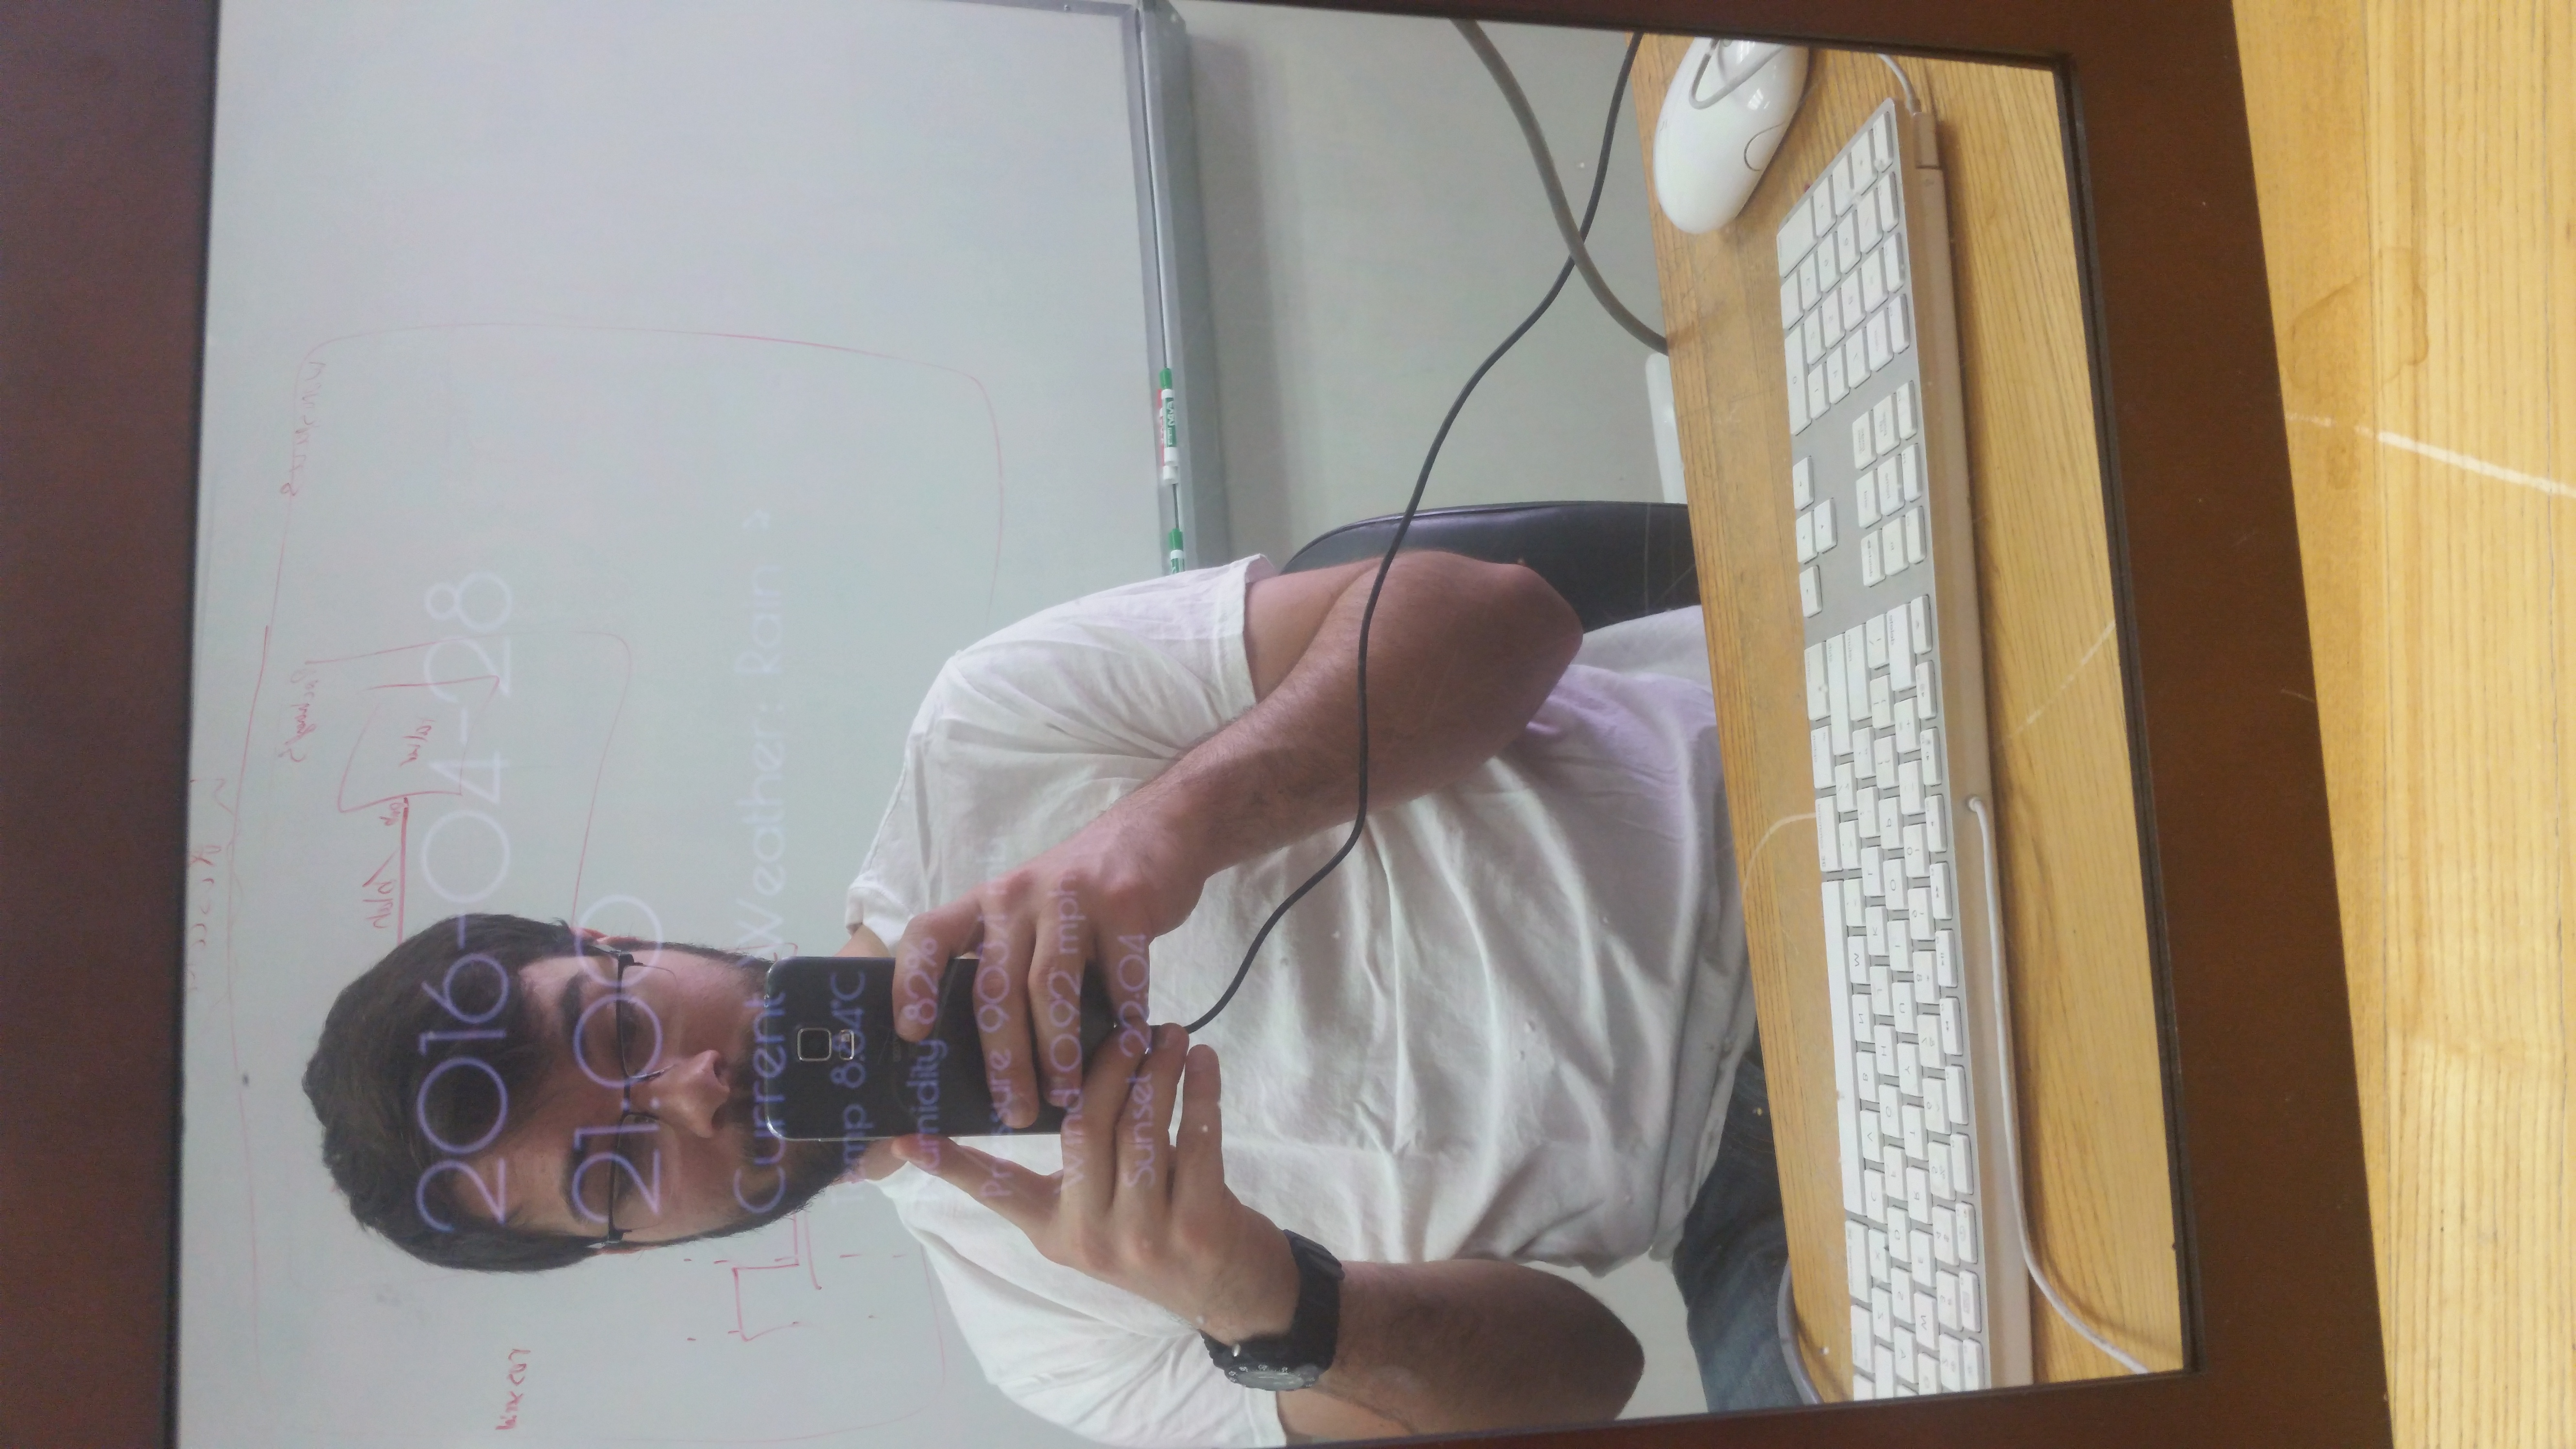
\includegraphics[width=2.5in, angle=-90]{images/Mirror.jpg}
  \caption{The finished Magic Mirror in action. Note the displayed text which appears near the dark regions of the photo.}
  \label{fig:mirror}
\end{figure}


\section{Related Work}  
%An academic paper should demonstrate novelties, i.e., things and/or theories that have not been done in the whole world. This requires the authors to be familiar with the complete bibliography. The most related work to this paper should be presented in this section. Comparison should be made whenever necessary to demonstrate the difference between this work and related work.
%REMEMBER TO CITE!!!!


%%% Harun, you need to find the original project that this is based on and cite it.
%%% also talk about how our project differs from that original project.
This project was inspired by an already existing work of \href{http://michaelteeuw.nl/}{Michael Teeuw}. The hardware implementation we followed can be seen using this link \href{http://michaelteeuw.nl/post/80391333672/magic-mirror-part-i-the-idea-the-mirror}{Mr.Teeuw}. As we went along with the implementation we came across an idea of including a PIR sensor. By employing PIR we can detect the human presence , thereby automating the screen to turn on and off when someone stands infront of it. This not only provides a futuristic feature but also conserves energy . 



\section{System} 
%The name of this section can be the name of the actual system students are developing or other meaningful names. A detailed description of the system. The overall design of the system should be presented first, followed by detailed introduction to complicated components. Subsections should be used whenever necessary, for example, when the content is too long as one section/subsection.
Building the Magic Mirror consisted of two parts, building the device, and writing an inituitve web interface.
\subsection{Building the Magic Mirror}
The mirror that was constructed for this project was assembled using a variety of used electronics as shown in Table \ref{tab:cost}.


\begin{table}[!t]
% increase table row spacing, adjust to taste
\renewcommand{\arraystretch}{1.3}
%if using array.sty, it might be a good idea to tweak the value of
%\extrarowheight as needed to properly center the text within the cells
\caption{Parts List and Cost}
\label{tab:cost}
\centering
% Some packages, such as MDW tools, offer better commands for making tables
% than the plain LaTeX2e tabular which is used here.
\begin{tabular}{|l||c|}
\hline
Part Description & Cost\\
\hline
\hline
Raspberry PI & \$35\\
\hline
PIR Sensor & \$15\\
\hline
Small LCD Television & Free*\\
\hline
USB Wireless Card & \$5\\
\hline
Automotive Window Tint & \$10\\
\hline
Plexiglas & \$7\\
\hline
Used Picture Frame & \$5\\
\hline
Misc. Fasteners & \$10\\
\hline
\end{tabular}
\end{table}




\subsection{Programming the Magic Mirror}

\section{Analysis} 
%In the section of System, we focus on the big picture of the system and cover most issues that can be explained clearly. We often move heavy mathematical analysis of components and performance of the system into another section called Analysis or other appropriate names. 

\section{Evaluation}
%In this section, system performance is presented. How well does the system achieve its goal? Quantitative metrics should be used whenever necessary. Tables, figures with curves and charts are often used to show the performance such as the trend. To this end, 
  %whatever system students have developing, at least one week of data must be collected to show meaningful results. 
%For the alternative project on Edimax plug security, students should use Raspberry Pi to control the plug for at least one week and record the activities of turning on/off the plug with Raspberry Pi and other meaningful data.


%%% Peter, include the results of your data here with graph or table.
%%% examples of how to do this are shown below
%%% also talk about your results and what they mean

\subsection{Motion Detection}
In keeping with the Security and Privacy aspects of this course, a portion of our testing was dedicated to exploring exactly what kind of information a device such as the Magic Mirror could collect if it were deployed in, for example, a user's home.
To that end, we collected motion detection data from the device's PIR sensor over the course of one week in the workspace of one of our group members.
Figures \ref{fig:chart26} and \ref{fig:chart29} show, by way of example, the data collected on April 26 and April 29, 2016, respectively.
The vertical axis shows the number of positive detections reported by the PIR sensor, and these are bucketed into twelve two-hour periods for each day's histogram.
Even these examples yield information as to when this individual spent the most time at his desk, at which the motion sensor was pointed.
\begin{figure}[!ht]
  \centering
  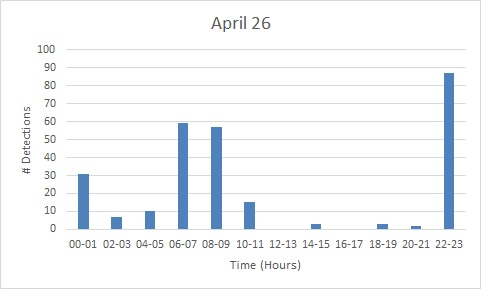
\includegraphics[width=2.75in]{images/Chart-April26.jpg}
  \caption{Histogram showing motion activity on April 26}
  \label{fig:chart26}
\end{figure}

\begin{figure}[!ht]
  \centering
  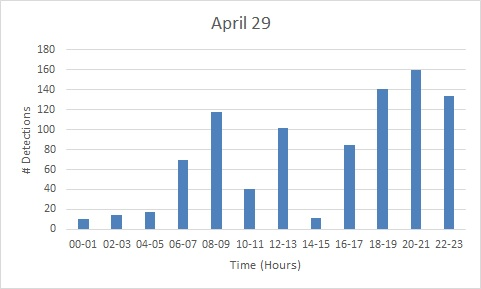
\includegraphics[width=2.75in]{images/Chart-April29.jpg}
  \caption{Histogram showing motion activity on April 29}
  \label{fig:chart29}
\end{figure}

By collecting this type of data over multiple days, we can begin to model the user's habits by calculating the average number of motion detections within a particular time interval over the course of the data collection period.
During our study spanning from April 24 to May 1 2016, we compiled a set of averages for each two-hour in the day. Figure \ref{fig:chartavg} plots these averages against their corresponding time intervals.
\begin{figure}[!ht]
  \centering
  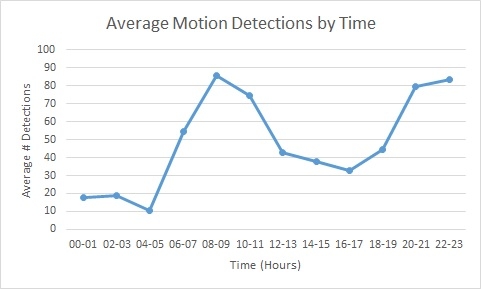
\includegraphics[width=2.75in]{images/Chart-averages.jpg}
  \caption{Average number of motion detections during each of 12 two-hour periods, from April 24 to May 1}
  \label{fig:chartavg}
\end{figure}

We can see in Figure \ref{fig:chartavg} that there are certain times when the user is relatively more likely to be moving within the field of view of the motion sensor.
In this case, 06 to 10 hours (6:00 AM to 10:00 AM) and 20 hours (8:00 PM) onward appear, on average, to be the times of greatest activity in this workspace.
Because the sensor senses at very short range, this places the individual within close proximity of the device itself.
As such, logging this data insecurely could compromise the privacy of the user by disclosing those times when the user is near the device, which could be used in conjunction with knowledge about the device's location to arrive at additional conclusions about that individual's daily routine.

\subsection{Mirror UI}
As the Magic Mirror's function is based largely on bringing aesthetically pleasing utility to a common wall fixture, our evaluation of the UI's success relies heavily upon the comments we received from those who observed the demonstration of the Magic Mirror during the final presentation session.
Those in attendance spoke favorably about the look and feel of the UI and the information it provides, with a few people noting that they would have use for a Magic Mirror of their own.
Figure \ref{fig:mirrorui} shows the Magic Mirror's informational UI for reference.
\begin{figure}[!ht]
  \centering
  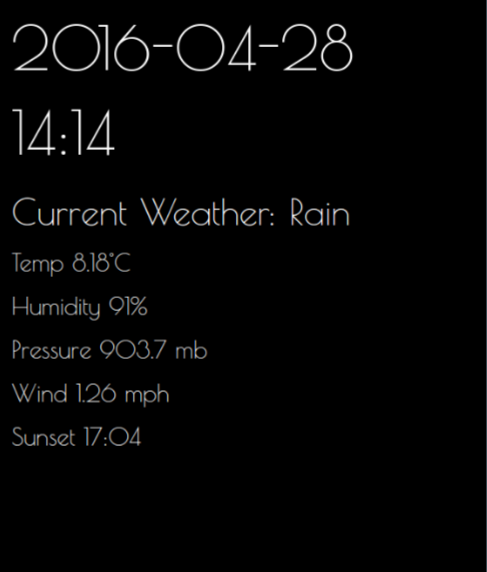
\includegraphics[width=2.75in]{images/mirror-ss.png}
  \caption{Screen capture of the Magic Mirror's information display UI}
  \label{fig:mirrorui}
\end{figure}


% An example of a floating figure using the graphicx package.
% Note that \label must occur AFTER (or within) \caption.
% For figures, \caption should occur after the \includegraphics.
% Note that IEEEtran v1.7 and later has special internal code that
% is designed to preserve the operation of \label within \caption
% even when the captionsoff option is in effect. However, because
% of issues like this, it may be the safest practice to put all your
% \label just after \caption rather than within \caption{}.
%
% Reminder: the "draftcls" or "draftclsnofoot", not "draft", class
% option should be used if it is desired that the figures are to be
% displayed while in draft mode.
%
%\begin{figure}[!t]
%\centering
%\includegraphics[width=2.5in]{myfigure}
% where an .eps filename suffix will be assumed under latex, 
% and a .pdf suffix will be assumed for pdflatex; or what has been declared
% via \DeclareGraphicsExtensions.
%\caption{Simulation results for the network.}
%\label{fig_sim}
%\end{figure}

% Note that the IEEE typically puts floats only at the top, even when this
% results in a large percentage of a column being occupied by floats.


% An example of a double column floating figure using two subfigures.
% (The subfig.sty package must be loaded for this to work.)
% The subfigure \label commands are set within each subfloat command,
% and the \label for the overall figure must come after \caption.
% \hfil is used as a separator to get equal spacing.
% Watch out that the combined width of all the subfigures on a 
% line do not exceed the text width or a line break will occur.
%
%\begin{figure*}[!t]
%\centering
%\subfloat[Case I]{\includegraphics[width=2.5in]{box}%
%\label{fig_first_case}}
%\hfil
%\subfloat[Case II]{\includegraphics[width=2.5in]{box}%
%\label{fig_second_case}}
%\caption{Simulation results for the network.}
%\label{fig_sim}
%\end{figure*}
%
% Note that often IEEE papers with subfigures do not employ subfigure
% captions (using the optional argument to \subfloat[]), but instead will
% reference/describe all of them (a), (b), etc., within the main caption.
% Be aware that for subfig.sty to generate the (a), (b), etc., subfigure
% labels, the optional argument to \subfloat must be present. If a
% subcaption is not desired, just leave its contents blank,
% e.g., \subfloat[].


% An example of a floating table. Note that, for IEEE style tables, the
% \caption command should come BEFORE the table and, given that table
% captions serve much like titles, are usually capitalized except for words
% such as a, an, and, as, at, but, by, for, in, nor, of, on, or, the, to
% and up, which are usually not capitalized unless they are the first or
% last word of the caption. Table text will default to \footnotesize as
% the IEEE normally uses this smaller font for tables.
% The \label must come after \caption as always.
%
%\begin{table}[!t]
%% increase table row spacing, adjust to taste
%\renewcommand{\arraystretch}{1.3}
% if using array.sty, it might be a good idea to tweak the value of
% \extrarowheight as needed to properly center the text within the cells
%\caption{An Example of a Table}
%\label{table_example}
%\centering
%% Some packages, such as MDW tools, offer better commands for making tables
%% than the plain LaTeX2e tabular which is used here.
%\begin{tabular}{|c||c|}
%\hline
%One & Two\\
%\hline
%Three & Four\\
%\hline
%\end{tabular}
%\end{table}


\section{Conclusion}
%In this section, the presented work is concluded. A brief introduction to the work is expected. Include the highlights of the work in conclusion. If necessary, future work can be discussed here.

% use section* for acknowledgment
%\section*{Acknowledgment}


% =====================================================  references section =======================================================
%References. At the end of the paper, there is always References. In the body of the paper, appropriate citations of references should be inserted into the right position, identifying related work. The list of references must not include references not cited in the paper. That is, references cannot be just listed without citations in the paper. Please use the reference and citation formatting in IEEE formatting template in this paper. 

% can use a bibliography generated by BibTeX as a .bbl file
% BibTeX documentation can be easily obtained at:
% http://mirror.ctan.org/biblio/bibtex/contrib/doc/
% The IEEEtran BibTeX style support page is at:
% http://www.michaelshell.org/tex/ieeetran/bibtex/
%\bibliographystyle{IEEEtran}
% argument is your BibTeX string definitions and bibliography database(s)
%\bibliography{IEEEabrv,../bib/paper}
%
% <OR> manually copy in the resultant .bbl file
% set second argument of \begin to the number of references
% (used to reserve space for the reference number labels box)
\begin{thebibliography}{1}

%\bibitem{IEEEhowto:kopka}
%H.~Kopka and P.~W. Daly, \emph{A Guide to \LaTeX}, 3rd~ed.\hskip 1em plus
 % 0.5em minus 0.4em\relax Harlow, England: Addison-Wesley, 1999.

\end{thebibliography}

\end{document}


